\documentclass{beamer}
\usepackage{textcomp} %textrightarrow
\usepackage{listings}
\usepackage{graphicx}
\usetheme{Boadilla}
\title{Visualizing the effects of compiler optimizations}
\author{Pietro Ghiglio}


\AtBeginSection[]
{
  \begin{frame}
    \frametitle{Table of Contents}
    \tableofcontents[currentsection]
  \end{frame}
}

\begin{document}
\titlepage

\begin{frame}
\frametitle{Table of Contents}
\tableofcontents
\end{frame}

\section{Introduction}

\begin{frame}
\frametitle{Background}
\begin{itemize}
\item I'm currently working on my thesis about source code-level visualization of the energy consumption of a program, using debug information. 
\item Compiler optimizations "obfuscate" the mapping between source code locations and assembly instructions. 
\item I needed to assess their impact on debug information, eventually "filling the gaps" they may have been left by compiler optimizations. 
\end{itemize}
\end{frame}

\begin{frame}
\frametitle{Background - 2}
I produced a tool that:
\begin{itemize}
\item Offers a view of the modules before and after a transformation pass has run, highlighting the differences.
\item Attempts to automatically propagate debug information when instructions are replaced by other instructions during transformation passes.
\end{itemize}
\end{frame}

\section{Visualization}

\begin{frame}
\frametitle{Dropdown menu}
Dropdown menu with the list of transformation passes that opt performed.
\begin{figure}[b]
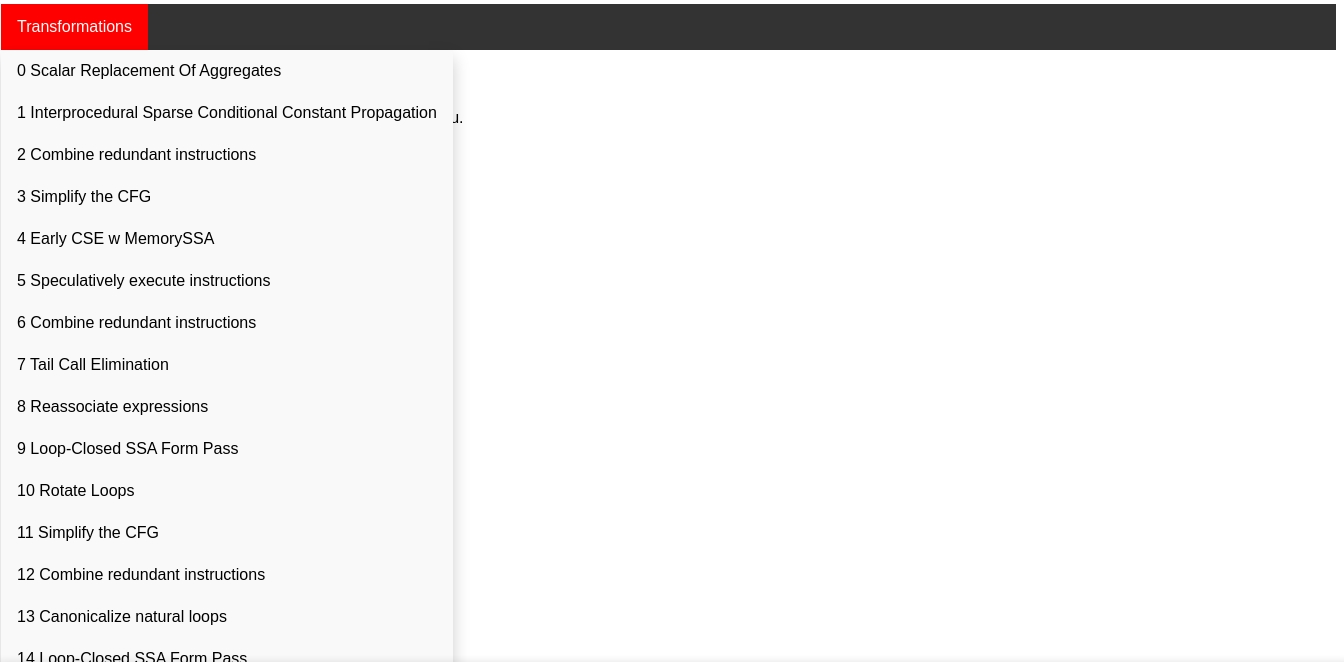
\includegraphics[scale=0.2]{dropdown.jpg}
\end{figure}
\end{frame}

\begin{frame}
\frametitle{Diff view}
For each pass, shows the module before and after the pass, highlighting the differences. \newline
\begin{figure}[b]
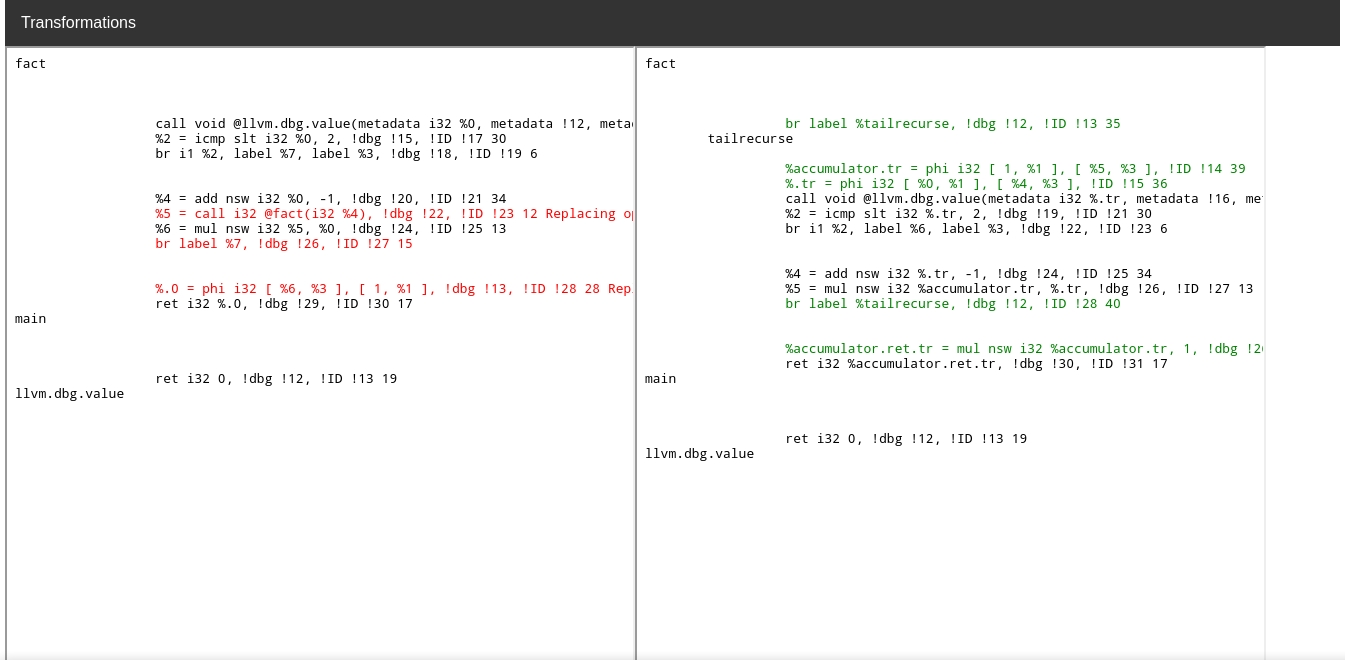
\includegraphics[scale=0.25]{ba.jpg}
\end{figure}
\end{frame}

\begin{frame}
\frametitle{Replaced information}
Displays information about the fact that an instruction has been replaced by another instruction, or that an instruction has been moved to a different location in the module.\newline
\begin{figure}[b]
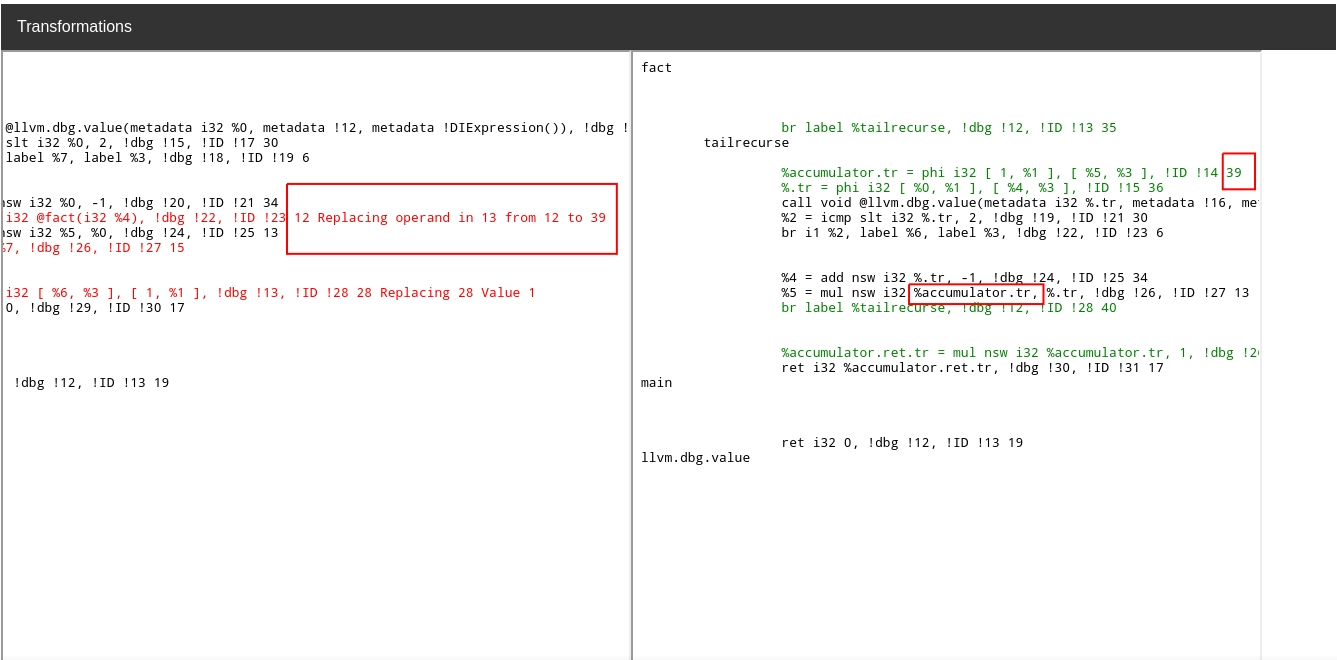
\includegraphics[scale=0.25]{rep.jpg}
\end{figure}
\end{frame}

\section{Debug info propagation}
\begin{frame}
\frametitle{Debug info propagation}
Using the information about whether an instruction has been replaced by another one, we can assign the debug location of the replaced instruction to the replacing one. \newline
\end{frame}

\begin{frame}
\frametitle{Example - Function inlining}
The two call instructions are replaced with the last operations of the inlined functions.
\begin{figure}[b]
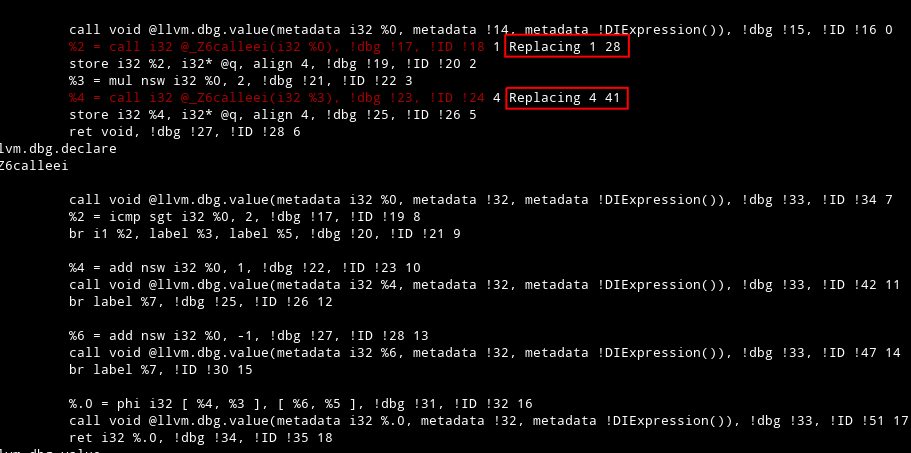
\includegraphics[scale=0.35]{pre_inline.png}
\end{figure}
\end{frame}

\begin{frame}
\frametitle{Example - Function inlining cont.}
The two phi-nodes do not have line/column information, but we can assign them the locations of the old call instructions that they replace.
\begin{figure}[b]
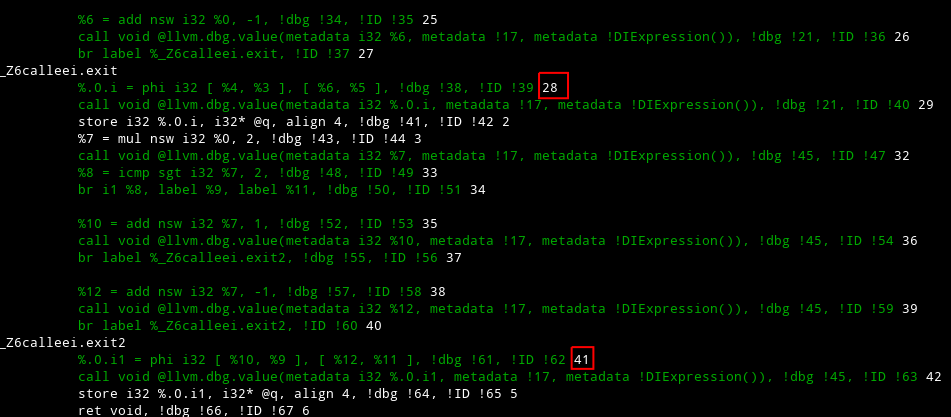
\includegraphics[scale=0.35]{post_inline.png}
\end{figure}
\end{frame}

\section{Implementation}

\begin{frame}
\frametitle{Workflow}
\begin{itemize}
\item I added a command line option to opt (-pn) that prints the module after each transformation (like -p) and logs all the operations performed by a pass (instruction creation, deletion, replacing and moving). 
\item Currently, I redirect this output to a file, and I've written a tool that parses it, propagates debug locations and outputs the html files.
\item I'm thinking about integrating the propagation and html files production directly into opt, removing the "redirect and parse" steps, which will speed up the entire process, removing the need of reading and writing to disk.
\end{itemize}
\end{frame}


\begin{frame}
\frametitle{Implementation}
Two (very simple) utility passes:
\begin{itemize}
\item -addUnique: adds a unique id the all the instructions in the module.
\item -printPassName: simply prints the name of the next pass in the pipeline (used to show pass names in the dropdown menu).
\end{itemize}
I've modified the LLVM functions for creating, removing, moving and replacing instructions, making them also produce a log entry of the performed operation. \newline
I also had to manually inspect the code of some transformation passes, adding log entries when needed.
\end{frame}

\section{Conclusion}
\begin{frame}
\frametitle{Final remarks}
\begin{itemize}
\item Showing the changes that a module underwent could have been done by simply "diffing" the string representations of the module. There's some work in that sense by the LLVM community (eg. check out the talk "Understanding Changes made by a Pass in the Opt Pipeline." at the last LLVM conference).
\item I needed something with a "deeper understanding" of what the transformation did, in order to automatically propagate debug information.
\item This required modifying the code of some of the core LLVM features, making my implementation a bit "heavy" from the point of view of maintenance and, eventually, distribution. But it could very well be a stand-alone tool.
\end{itemize}
\end{frame}









\end{document}